\documentclass{beamer}
\beamertemplatenavigationsymbolsempty
\usepackage[french]{babel}
\usepackage{fontspec}
\usepackage{amsmath, amsthm, amsfonts}
\usepackage[separate-uncertainty]{siunitx}
\usepackage{xcolor}
\usepackage{tikz}
\usepackage{tikz-cd}
\usepackage[object=vectorian]{pgfornament}
\usepackage{circuitikz}
\usepackage{hyperref}
\usepackage{caption}
\usepackage{booktabs}
\usepackage{mathtools}
\usepackage{longtable}
\usepackage[version=3]{mhchem}
\usepackage{marginnote}
\usepackage[framemethod=tikz]{mdframed}


% Paul Tol's qualitative palette
% ``bright''.https://personal.sron.nl/~pault/#sec:qualitative
\definecolor{tblue}{HTML}{4477AA}
\definecolor{tcyan}{HTML}{66CCEE}
\definecolor{tgreen}{HTML}{228833}
\definecolor{tyellow}{HTML}{CCBB44}
\definecolor{tred}{HTML}{EE6677}
\definecolor{tpurple}{HTML}{AA3377}
\definecolor{tgrey}{HTML}{BBBBBB}


% Justification for marginnotes.
\renewcommand*{\raggedleftmarginnote}{}
\renewcommand*{\raggedrightmarginnote}{}


% Styles for mdframed environments.
\newmdenv[backgroundcolor=tgreen!10,linecolor=tgreen!30]{reponsebox}
\newmdenv[backgroundcolor=tyellow!10,linecolor=tyellow!30]{diapobox}
\newmdenv[backgroundcolor=tred!10,linecolor=tred!30]{fondamentalbox}

% Default arrow for tikz and style for positive and negative objects.
\tikzset{>=latex,
    negative/.style={draw=teal!70!black, fill=teal!10, thick},
    positive/.style={draw=red, fill=red!10, thick}}
\usetikzlibrary{matrix,calc,decorations.pathreplacing,decorations.pathmorphing,decorations.markings}

% French locale for numbers and negative exponent for units.
\sisetup{locale=FR, per-mode=symbol}

\newcommand{\abs}[1]{\left| #1 \right|}
\newcommand{\rhat}{\vec{\hat{r}}}
\newcommand{\xhat}{\vec{\imath}}
\newcommand{\yhat}{\vec{\jmath}}
\newcommand{\zhat}{\vec{k}}
\newcommand{\real}{\mathbb{R}}
\newcommand{\der}[2]{\frac{\mathrm{d}#1}{\mathrm{d}#2}}
\newcommand{\pder}[2]{\frac{\partial\ #1}{\partial\ #2}}
\newcommand{\dif}{\mathrm{d}}
\newcommand{\ddif}{\,\mathrm{d}}
\newcommand{\grad}{\vec{\nabla}}
\newcommand{\exemple}[1]{\begin{fullwidth}#1\end{fullwidth}}
\newcommand{\norm}[1]{\lVert\ #1\ \rVert}
\newcommand{\vu}{\vec{u}}
\newcommand{\vv}{\vec{v}}
\newcommand{\vr}{\vec{r}}
\newcommand{\va}{\vec{a}}
\newcommand{\vF}{\vec{F}}
\newcommand{\vE}{\vec{E}}
\newcommand{\vB}{\vec{B}}
\newcommand{\vecxyz}[3]{#1 \xhat\ + #2 \yhat\ + #3 \zhat}
\newcommand{\vecxy}[2]{#1 \xhat\ + #2 \yhat}
\newcommand{\coulombcst}{k}
\newcommand{\emf}{\ensuremath{\mathcal{E}}}
\newcommand{\eval}{\SI{1.602e-19}{C}}
\newcommand{\kval}{\SI{8.99e9}{Nm^2 \per C^2}}

% Nice separator line
\newcommand{\sectionline}{
    \noindent
    \begin{center}
        \resizebox{0.5\linewidth}{1ex}
    {{%
    {\begin{tikzpicture}
    \node  (C) at (0,0) {};
    \node (D) at (9,0) {};
    \path (C) to [ornament=85] (D);
    \end{tikzpicture}}}}
    \end{center}
}

\theoremstyle{definition}
\newtheorem*{defn}{Definition}


\usepackage[version=3]{mhchem}

\setbeamercolor{title}{fg=tblue}
\setbeamercolor{frametitle}{fg=tblue}
\setbeamercolor{structure}{fg=tblue}

% Make footnotesize smaller
\makeatletter
\renewcommand\footnotesize{%
   \@setfontsize\footnotesize\@viipt{11}%
   \abovedisplayskip 8\p@ \@plus2\p@ \@minus4\p@
   \abovedisplayshortskip \z@ \@plus\p@
   \belowdisplayshortskip 4\p@ \@plus2\p@ \@minus2\p@
   \def\@listi{\leftmargin\leftmargini
               \topsep 4\p@ \@plus2\p@ \@minus2\p@
               \parsep 2\p@ \@plus\p@ \@minus\p@
               \itemsep \parsep}%
   \belowdisplayskip \abovedisplayskip
}
\makeatother

\title{Électricité et magnétisme}
\subtitle{Chapitre 2 - Champ électrique}
\date{31 août 2021}
\author{Loïc Séguin-Charbonneau}
\institute{Cégep Édouard-Montpetit}


\begin{document}

\maketitle


\begin{frame}[t]{Déduire le champ à partir de la force}
  On place une charge de \SI{4.00}{nC} à un endroit $P$. Elle subit une force
  de \SI{24.0}{\micro N} vers la gauche.

  \vspace{\baselineskip}

  \only<1-2>{
    Quel est la direction du champ électrique au point $P$?
    \begin{enumerate}[A.]
      \item<alert@2> vers la gauche
      \item vers le bas
      \item vers la droite
      \item vers le haut
    \end{enumerate}
  }

  \only<3-4>{
    Quel est la grandeur du champ électrique au point $P$?
    \begin{enumerate}[A.]
      \item \SI{96.0e-15}{N C}
      \item \SI{0.167e-3}{C/N}
      \item<alert@4> \SI{6.00e3}{N/C}
      \item \SI{0.167e3}{N/C}
    \end{enumerate}
  }
  \only<5-6>{
    Quel est le champ électrique au point $P$ si on enlève la charge de
    \SI{4.00}{nC}?
    \begin{enumerate}[A.]
      \item<alert@6> \SI{6.00e3}{N/C} vers la gauche
      \item \SI{6.00e3}{N/C} vers la droite
      \item nul
      \item \SI{-2.00e3}{N/C}
    \end{enumerate}
  }
  \only<7-8>{
    Quelle serait la force sur une particule de charge \SI{-2.00}{nC} placée
    au même endroit?
    \begin{enumerate}[A.]
      \item \SI{24.0}{\micro N} vers la gauche
      \item \SI{24.0}{\micro N} vers la droite
      \item \SI{48.0}{\micro N} vers la droite
      \item<alert@8> \SI{12.0}{\micro N} vers la droite
    \end{enumerate}
  }
\end{frame}


\begin{frame}[t]{Électrophorèse sur gel}
\begin{columns}
  \column{0.5\textwidth}
  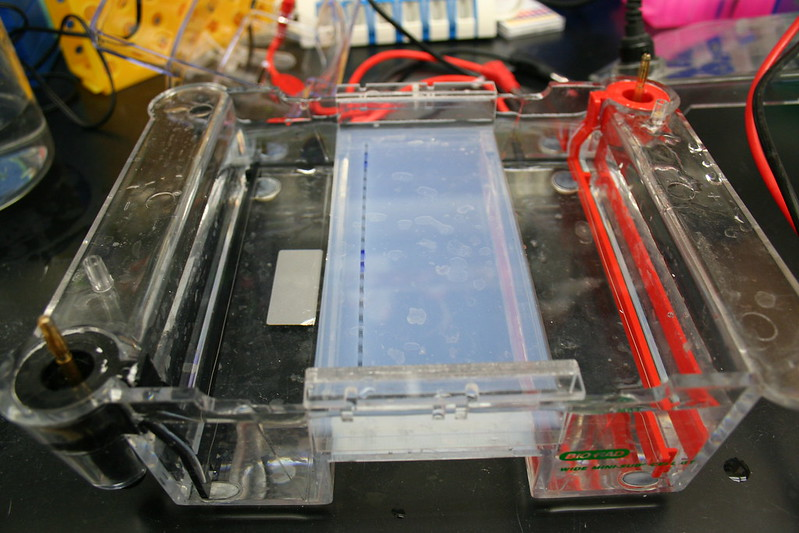
\includegraphics[width=\textwidth]{figures/gel_electrophoresis.jpg}
  \\
  \footnotesize \href{https://www.flickr.com/photos/34857812@N04/3235838168}{PlaxcoLab} (CC BY-2.0)

  \column{0.5\textwidth}
  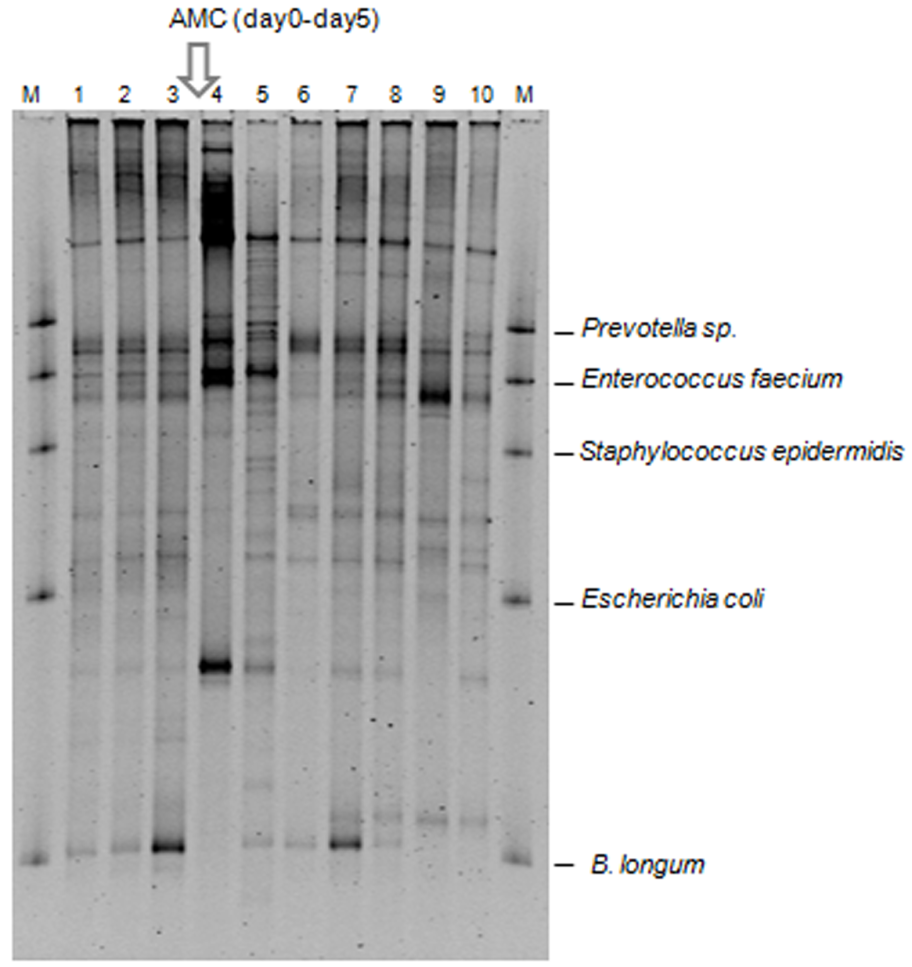
\includegraphics[width=\textwidth]{figures/electrophoresis_mangin_et_al.png}
  \\
  \footnotesize Mangin I, Lévêque C, Magne F, Suau A, Pochart P (2012)
  Long-Term Changes in Human Colonic Bifidobacterium Populations Induced by a
  5-Day Oral Amoxicillin-Clavulanic Acid Treatment. PLoS ONE 7(11): e50257.
  https://doi.org/10.1371/journal.pone.0050257

\end{columns}
\end{frame}


\begin{frame}[t]{Électrophorèse sur gel}
  On place des fragments d'ADN dans un appareil d'électrophorèse sur gel et on
  active un champ électrique de \SI{500}{\newton\per\coulomb}. La densité de
  charge de l'ADN est environ \SI{-942}{\pico\coulomb\per\meter}. La densité de
  masse est de \SI{3.155e-21}{\gram\per\meter}.

  \vspace{\baselineskip}
  \only<1-2>{
    Quelle est la grandeur de la force électrique sur un fragment d'ADN de
    \SI{10.0}{\micro\meter}?

    \begin{enumerate}[A.]
      \item \SI{4.71e-7}{\newton}
      \item<alert@2> \SI{4.71e-12}{\newton}
      \item \SI{1.486e-27}{\newton}
      \item \SI{5.308e11}{\newton}
    \end{enumerate}
  }

  \only<3-4>{
    En supposant que la force électrique est la seule force en jeu, quelle
    serait la grandeur de l'accélération du fragment d'ADN?

    \begin{enumerate}[A.]
      \item \SI{9.8}{\meter\per\second\squared}
      \item \SI{6.31e-24}{\meter\per\second\squared}
      \item<alert@4> \SI{1.493e17}{\meter\per\second\squared}
      \item \SI{1.486e-32}{\meter\per\second\squared}
    \end{enumerate}
  }
\end{frame}


\begin{frame}{Champ électrique d'une charge ponctuelle}
  \[
    \vE = \frac{1}{4\pi\varepsilon_0} \frac{q}{r^2} \vu_r
  \]
  \begin{center}
  \begin{tikzpicture}[ampersand replacement=\&]
    \matrix[column sep=1.5cm] {
    \node[positive, circle] (q) at (0, 0) {$+$};
    \foreach \theta in {0, 30, ..., 330} {
      \draw[->] (q) -- ++(\theta:1);
      \draw[->] ($(q) + (\theta:1.05)$) -- ++(\theta:0.5);
      \draw[->] ($(q) + (\theta:1.05) + (\theta:0.55)$) -- ++(\theta:0.25);
    }
    \&
    \node[negative, circle] at (0, 0) {$-$};
    \foreach \theta in {0, 30, ..., 330} {
      \draw[<-] (q) -- ++(\theta:1);
      \draw[<-] ($(q) + (\theta:1.05)$) -- ++(\theta:0.5);
      \draw[<-] ($(q) + (\theta:1.05) + (\theta:0.55)$) -- ++(\theta:0.25);
    }
    \\
    };
  \end{tikzpicture} 
  \end{center}
\end{frame}


%\begin{frame}{Exercice}
  %Dans chacune des situations ci-dessous, utilisez les informations fournies
  %pour trouver la direction du champ électrique à la position de la charge de
  %droite.

  %\begin{columns}
    %\column{0.6\textwidth}
    %\begin{enumerate}
      %\item 
        %\begin{tikzpicture}
          %\node[positive, circle] (q1) at (0, 0) {$+$};
          %\node[positive, circle] (q2) at (2, 0) {$+$};
        %\end{tikzpicture}
      %\item 
        %\begin{tikzpicture}
          %\node[positive, circle] (q1) at (0, 0) {$+$};
          %\node[negative, circle] (q2) at (2, 0) {$-$};
        %\end{tikzpicture}
      %\item 
        %\begin{tikzpicture}
          %\node[negative, circle] (q1) at (0, 0) {$-$};
          %\node[positive, circle] (q2) at (2, 0) {$+$};
        %\end{tikzpicture}
      %\item 
        %\begin{tikzpicture}
          %\node[draw, circle] (q1) at (0, 0) {$q$};
          %\node[negative, circle] (q2) at (2, 0) {$-$};
          %\draw[very thick, ->] (q2) -- ++(1.5, 0) node[right] {$\vec{F}$};
        %\end{tikzpicture}
      %\item 
        %\begin{tikzpicture}
          %\node[positive, circle] (q1) at (0, 0) {$+$};
          %\node[draw, circle] (q2) at (2, 0) {$q$};
          %\draw[very thick, ->] (q2) -- ++(-1.5, 0) node[below] {$\vec{F}$};
        %\end{tikzpicture}
    %\end{enumerate}

    %\column{0.4\textwidth}
    %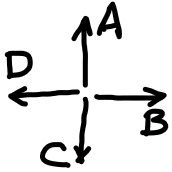
\includegraphics[width=0.5\textwidth]{figures/roseabcd.png}
  %\end{columns}
%\end{frame}


\begin{frame}{Exercice}
  Une charge $q = \SI{30}{\micro\coulomb}$ est placée à \SI{160}{cm} du sol. À
  droite de cette charge, une charge $Q = \SI{-50}{\micro\coulomb}$ est placée
  à \SI{2}{m} au-dessus du sol. La distance entre les deux charges est $D =
  \SI{3}{m}$.

  Calculer le champ électrique au point $P$ situé à \SI{1}{m} à droite de la
  charge $q$ et à \SI{4}{m} au-dessus du sol.

  \begin{center}
    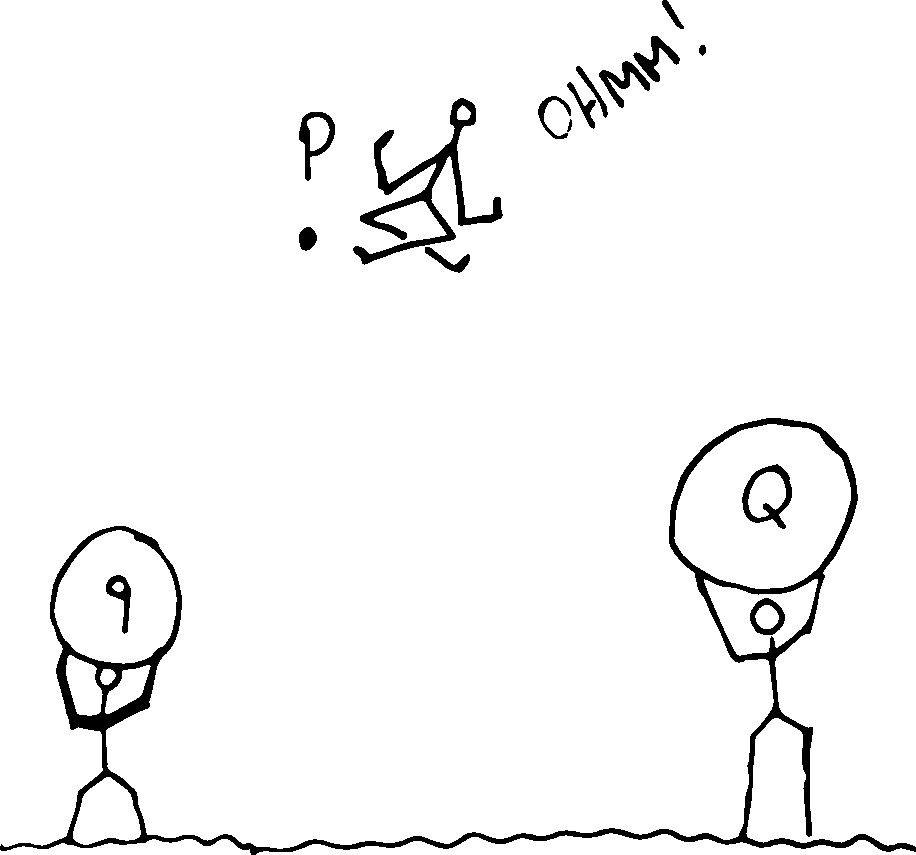
\includegraphics[scale=0.3]{figures/champ-deux-charges-1.pdf}
  \end{center}
\end{frame}


\begin{frame}[t]{Exercice lignes de champ}

  \begin{center}
    \begin{tikzpicture}
      \node[align=center] at (0, 0) {
        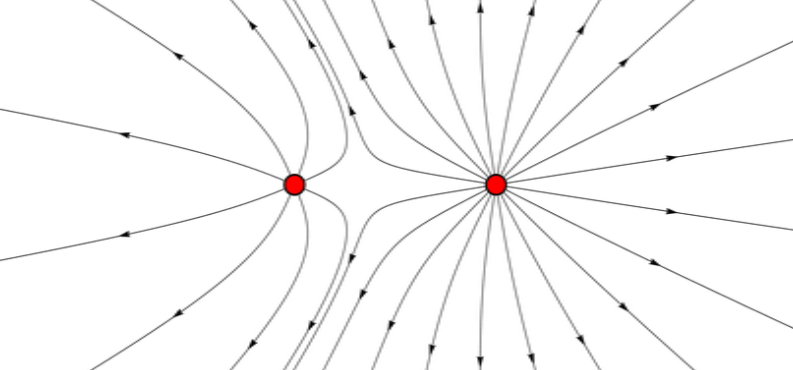
\includegraphics[scale=0.4]{figures/efield-ex0.png}
        \\
        \footnotesize{\url{https://www.st-andrews.ac.uk/~physapps/fande/Electric_Field_Lines.html}}
      };
      \only<5->{
        \draw[fill] (1.6, 1) circle (1pt) node[above] {\textbf{A}};
        \draw[fill] (2.2, 1.3) circle (1pt) node[above] {\textbf{B}};
        \draw[fill] (-2, -0.4) circle (1pt) node[above] {\textbf{C}};
        \draw[fill] (-0.3, 0.3) circle (1pt) node[above] {\textbf{D}};
      }
    \end{tikzpicture}
  \end{center}

  \only<1-2>{
    Quels sont les signes des deux charges?
    \begin{enumerate}[A.]
      \item $-$, $-$
      \item $-$, $+$
      \item $+$, $-$
      \item<alert@2> $+$, $+$
    \end{enumerate}
  }

  \only<3-4>{
  Laquelle des deux charges est la plus grande en valeur absolue?
  \begin{enumerate}[A.]
    \item celle de gauche
    \item<alert@4> celle de droite
    \item elles sont de même grandeur
  \end{enumerate}
  }

  \only<5-6>{
    Où le champ électrique est-il le plus grand?
  }
\end{frame}


\begin{frame}{Distribution de charge}
  Chaque disque et l'anneau ont tous la même charge $Q$.
  Classer les objets en ordre croissant de la grandeur du champ électrique au
  point $P$.

  \begin{center}
  \begin{tikzpicture}
    \matrix[row sep=1em, column sep=1em, ampersand replacement=\&] {
    \node at (0, -2.5) {(a)};
    \fill (0, 1.5) circle(1pt);
    \node[left] at (0, 1.5) {$P$};
    \draw (0,-2) -- (0,0);
    \draw[fill=black!10] (0,0) ellipse[x radius=1, y radius=0.5];
    \draw (0,0) -- (0,2);
    \draw (0,0) -- ++(-30:0.75);
    \node at (5:0.5) {$R$}; \&
    \node at (0, -2.5) {(b)};
    \fill (0, 1.5) circle(1pt);
    \node[left] at (0, 1.5) {$P$};
    \draw (0,-2) -- (0,0);
    \draw[fill=black!10] (0,0) ellipse[x radius=2, y radius=1];
    \draw (0,0) -- (0,2);
    \draw (0,0) -- ++(-30:1.5);
    \node at (-05:0.8) {$2R$}; \&
    \fill (0, 1.5) circle(1pt);
    \node[left] at (0, 1.5) {$P$};
    \node at (0, -2.5) {(c)};
    \draw (0,-2) -- (0,0);
    \draw[fill=black!10] (0,0) ellipse[x radius=2, y radius=1]; 
    \draw[fill=white] (0,0) ellipse[x radius=1, y radius=0.5];
    \draw (0,-0.5) -- (0,2);
    \draw (0,0) -- ++(-150:0.75);
    \node at (180:0.5) {$R$};
    \draw (0,0) -- ++(-30:1.5);
    \node at (-10:1.4) {$2R$};\\
    };
  \end{tikzpicture}
  \end{center}
\end{frame}


\begin{frame}{Tige divisée en $n$ sous-tiges}
\begin{columns}
  \column{0.3\textwidth}
  {\scriptsize
  \begin{center}
    \begin{tabular}{SS}
      \toprule
      $n$    &  {$E_x$ (\si{\newton\per\coulomb})}  \\
      \midrule
       1    &   -3714.9  \\
       2    &   -4343.9  \\
       3    &   -4516.8  \\
       4    &   -4585.4  \\
       5    &   -4619.1  \\
       6    &   -4637.9  \\
       7    &   -4649.4  \\
       8    &   -4657.0  \\
       9    &   -4662.3  \\
      10    &   -4666.0  \\
      11    &   -4668.8  \\
      12    &   -4671.0  \\
      13    &   -4672.6  \\
      14    &   -4674.0  \\
      15    &   -4675.0  \\
      16    &   -4675.9  \\
      17    &   -4676.6  \\
      18    &   -4677.2  \\
      19    &   -4677.8  \\
      20    &   -4678.2  \\
      \bottomrule
    \end{tabular}
  \end{center}
  }

  \column{0.7\textwidth}
  \begin{tikzpicture}[scale=0.8]
    \begin{axis}[
      xlabel={$n$},
      ylabel={$E_x$ (\si{\newton\per\coulomb})},
      font={\sffamily},
      /pgf/number format/.cd,
              use comma,
              1000 sep={}
    ]
      \addplot+[tblue, mark size=1pt] table {champ_n.dat};
    \end{axis}
  \end{tikzpicture}
\end{columns}
\end{frame}


\begin{frame}[t]{Champ d'un plan infini}
  \begin{columns}[t]
    \column{0.6\textwidth}
    Une plaque de métal de \SI{2.00}{\meter\squared} porte une charge totale de
    \SI{4.00}{\micro\coulomb}. 

    \only<1-2>{
      Quelle est la densité de charge de cette plaque?

      \begin{enumerate}[A.]
        \item<alert@2> \SI{2.00e-6}{\coulomb\per\meter\squared}
        \item \SI{0.500e6}{\coulomb\per\meter\squared}
        \item \SI{-2.00e-6}{\coulomb\per\meter\squared}
        \item \SI{-0.500e-6}{\coulomb\per\meter\squared}
      \end{enumerate}
    }
    \only<3-4>{
      Quel est la grandeur du champ électrique au point $P$ situé à
      \SI{8.00}{\centi\meter} au-dessus du plan?
      \begin{enumerate}[A.]
        \item \SI{225.9e3}{\newton\per\coulomb}
        \item<alert@4> \SI{112.9e3}{\newton\per\coulomb}
        \item \SI{5.619e6}{\newton\per\coulomb}
        \item \SI{561.9}{\newton\per\coulomb}
      \end{enumerate}
    }
    \only<5-6>{
      On ajoute une charge de \SI{80}{\nano\coulomb} à \SI{8.00}{\centi\meter}
      du plan, \SI{3.00}{\centi\meter} à droite du point $P$. Quel est
      maintenant le champ électrique au point $P$?

      \begin{enumerate}[A.]
        \item<alert@6> $\left(\num{-799.1} \yhat + \num{112.9} \zhat \right)\times 10^3 \si{\newton\per\coulomb}$
        \item $\SI{912.1e3}{\newton\per\coulomb} \zhat$
        \item $\left(\num{112.9} \yhat + \num{799.1} \zhat \right)\times 10^3 \si{\newton\per\coulomb}$
        \item $\left(\num{-799.1} \xhat + \num{112.9} \zhat \right)\times 10^3 \si{\newton\per\coulomb}$
      \end{enumerate}
    }

    \column{0.4\textwidth}
    \begin{center}
      \begin{tikzpicture}[scale=0.6]
        \draw (0, 0) -- (5, 0) -- (7, 3) -- (2, 3) -- cycle;
        \onslide<3->{
          \draw[densely dashed] (3, 1.5) -- (3, 4) node[left] {$P$};
          \fill (3, 4) circle (2pt);
        }
        \onslide<5->{
          \node[draw, circle] (q) at (5, 4) {$q$};
          \draw[densely dashed] (5, 1.5) -- (q);
          \draw[tblue, <->] (4.5, -1) node[left] {$z$} -- (4.5, -2)
             -- (5.5, -2) node[below] {$y$};
          \draw[tblue, ->] (4.5, -2) -- (4, -2.75) node[anchor=north east] {$x$};
        }
      \end{tikzpicture}
    \end{center}
  \end{columns}
\end{frame}

\begin{frame}{Tube à rayon cathodique}
  \begin{center}
    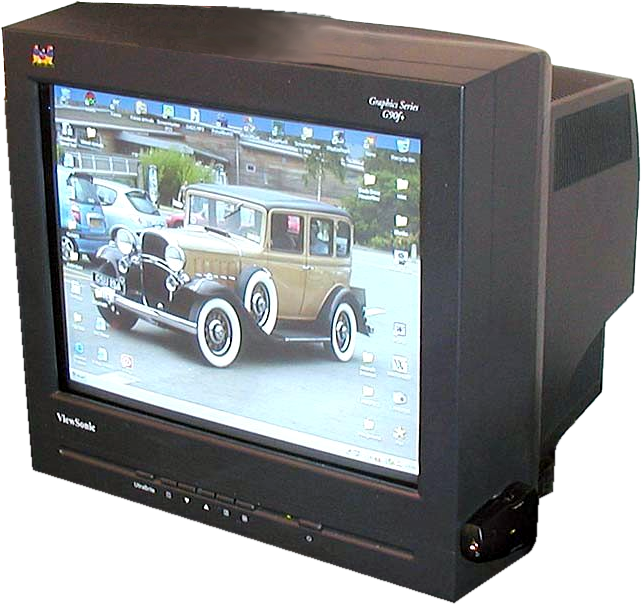
\includegraphics[scale=0.2]{figures/viewsonic-crt.png}
  \end{center}
\end{frame}


\begin{frame}{Tube à rayon cathodique}

  \begin{center}
  \begin{tikzpicture}[>=stealth, scale=0.8]
    \draw plot[smooth cycle] coordinates {(0, 1) (2, 1.5) (6, 3) (6, -3) (2, -1.5) (0, -1)};
    \draw[ultra thick] (0.8, 0.5) -- (2.5, 0.5);
    \draw[ultra thick] (0.8, -0.5) -- (2.5, -0.5);
    \foreach \x in {1.1, 1.5, 1.9, 2.3} {
      \node at (\x, 0.7) {$+$};
      \node at (\x, -0.7) {$-$};
    }
    \draw[thick, blue] plot[smooth] coordinates {(0, 0) (0.8, 0) (1.2, 0.02) (1.6, 0.04) (2, 0.08) (2.4, 0.16) (2.6, 0.2)} -- (6.4, 1.5);
    \draw[|<->|] (7, 3) -- node[fill=white] {$D$} (7, -3);
    \draw[|<->|] (0.8, -1.1) -- node[fill=white] {$l$} (2.5, -1.1);
    \draw[<->|] (2.5, -1.1) -- node[fill=white] {$L$} (6.4, -1.1);
  \end{tikzpicture}
  \end{center}

  Les dimensions du tube sont $l = \SI{2}{\centi\meter}$, $L =
  \SI{40}{\centi\meter}$ et $D = \SI{60}{\centi\meter}$.  Avant de passer entre
  les plaques du déflecteur, la vitesse des électrons est
  5\% de la vitesse de la lumière vers la droite.

  Déterminer la norme du champ électrique nécessaire pour que les électrons
  atteignent le haut de l'écran.

\end{frame}


\end{document}
